\section{Week 1: Introduction}
\begin{minipage}{.45\textwidth}
\textbf{A variety of tools in KRR:}
    \begin{itemize}
        \item Propositional logic (PL)
        \item First-order logic (FOL)
        \item Answer-Set Programming (ASP)
        \item Description logics (DL)
    \end{itemize}
\end{minipage}
\begin{minipage}{.45\textwidth}
  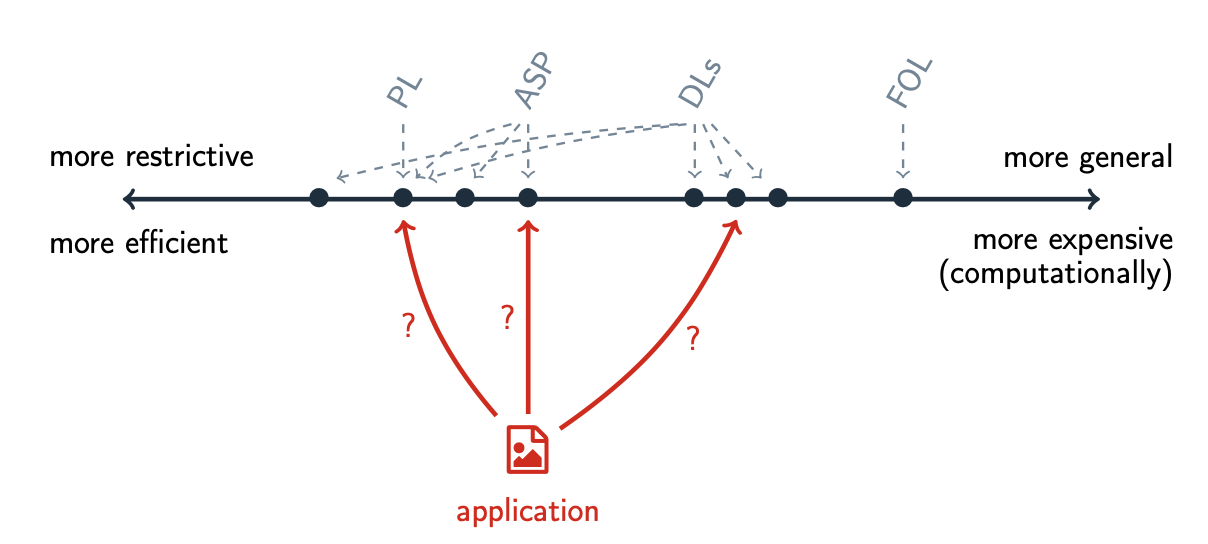
\includegraphics[scale=0.4]{figures/tradeoff.png}
%   \caption{Tradeoff tools KRR}
\end{minipage}
\vspace{1cm}

\subsection{Propositional Logic (PL) - $\vee$} 
\textcolor{red}{Propositional variables} represent statements that can be \textbf{true} or \textbf{false}. \\
\textcolor{red}{Logical operators} are used to build more complex statements: $\wedge, \vee, \neg, \rightarrow$.

\begin{itemize}
    \item[--] \textbf{Syntax of propositional logic}
    \begin{itemize}
        \item[$\circ$] Take some (infinite) set P of \textcolor{red}{propositional variables} $\rightarrow$ P = $\{p_1, p_2, \cdots \}$
        \item[$\circ$] Propositional logic \textcolor{blue}{formulas} construction:
        \begin{itemize}
            \item Each p $\in$ P is a \textcolor{blue}{formula}.
            \item If $\varphi$ is a \textcolor{blue}{formula}, then $\neg \varphi$ is a \textcolor{blue}{formula} too.
            \item If $\varphi_1, \varphi_2$ are \textcolor{blue}{formulas}, then so are $(\varphi_1 \wedge \varphi_2), \; (\varphi_1 \vee \varphi_2), \; (\varphi_1 \rightarrow \varphi_2)$ and $(\varphi_1 \leftrightarrow \varphi_2)$.
        \end{itemize}
        \item[$\circ$] \textit{Example propositional logic formula:}
        $(p_1 \vee p_2 \vee p_3) \leftrightarrow \left(\neg p_1 \rightarrow (p_2 \vee p_3)\right)$
    \end{itemize}
    \item[--] \textbf{Semantics of propositional logic}
    \begin{itemize}
        \item[$\circ$] Let $\varphi$ be a prop. logic formula that contains variables $p_1, \cdots, p_n$
        \item[$\circ$] Consider \textcolor{red}{truth assignments} $\alpha: P \rightarrow \{0,1\}$, where \textcolor{red}{0} = \textcolor{red}{false} and \textcolor{ForestGreen}{1} = \textcolor{ForestGreen}{true}.
        \item[$\circ$] When a \textcolor{red}{truth assignment} $\alpha$ makes a \textcolor{blue}{formula} $\varphi$ true, \textbf{or} when it satisfies $\varphi$, written $\alpha \models \varphi$ \\
        \\
        \textbf{iff = if and only if} \\
        \begin{minipage}{.45\textwidth}
        \vspace{0.15cm}
            \begin{itemize}
                \item \textcolor{RoyalBlue}{$\alpha \models p$} iff $\alpha(p) = 1$
                \item \textcolor{RoyalBlue}{$\alpha \models \varphi_1 \wedge \varphi_2$} iff both $\alpha \models \varphi_1$ and $\alpha \models \varphi_2$
                \item \textcolor{RoyalBlue}{$\alpha \models \varphi_1 \wedge \varphi_2$} iff $\alpha \models \varphi_1$ or $\alpha \models \varphi_2$ (or both)
            \end{itemize}
        \end{minipage}
        \begin{minipage}{.45\textwidth}
        \vspace{0.15cm}
            \begin{itemize}
                \item \textcolor{RoyalBlue}{$\alpha \models \neg \varphi$} iff $\alpha \not \models \varphi$
                \item \textcolor{RoyalBlue}{$\alpha \models \varphi_1 \rightarrow \varphi_2$} iff $\alpha \models (\neg \varphi_1) \vee \varphi_2$
                \item \textcolor{RoyalBlue}{$\alpha \models \varphi_1 \leftrightarrow \varphi_2$} iff $\alpha \models (\varphi_1 \rightarrow \varphi_2) \wedge (\varphi_2 \rightarrow \varphi_1)$
            \end{itemize}
        \end{minipage}
    \end{itemize}
    \newpage
    \item[--] \textbf{Conjunctive Normal Form (CNF)}
    \begin{itemize}
        \item[$\circ$] Useful to consider only formulas of a particular (\textbf{normal}) form.
        \item[$\circ$] A \textbf{CNF formula} is the conjunction ($\wedge$) of several clauses
        \begin{itemize}
            \item A \textcolor{blue}{literal} is a propositional variable $p$ or the negation $\neg p$ of a variable
            \item A \textcolor{OrangeRed}{clause} is the disjunction ($\vee$) of several \textcolor{blue}{literals}
            \item \textit{Example:} $(p_1 \vee \neg p_2) \wedge (p_1 \vee p_2) \wedge (\neg p_1 \vee p_3 \vee \neg p_4)$
            \\
            \item \textit{Every propositional logic formula can be equivalently expressed as a \textbf{CNF formula}}.
        \end{itemize}
    \end{itemize}
    \item[--] \textbf{Reasoning tasks}
    \begin{itemize}
        \item[$\circ$] \textcolor{red}{Satisfiability:}
        Given a formula $\varphi$, does there exist a truth assignment $\alpha$ that satisfies $\varphi$?
        \begin{itemize}
            \item \textcolor{red}{Satisfiability} can be \textbf{reduced to} \textcolor{red}{non-entailment}: \\
            $\varphi$ is \textcolor{red}{satisfiable} iff $\varphi \not \models (p_1 \wedge \neg p_2)$
        \end{itemize}
        \item[$\circ$] \textcolor{NavyBlue}{Entailment:}
        Given two formulas $\varphi_1, \varphi_2$, does it hold that $\varphi_1$ entails $\varphi_2$, written as $\varphi_1 \models \varphi_2$? \\
        
        $\varphi_1 \models \varphi_2$ iff for all assignments $\alpha$ such that $\alpha \models \varphi_1$ and $\alpha \models \varphi_2$. \\
        (\textit{Intuitively:} if one assumes that $\varphi_1$ is true, then $\varphi_2$ must also be true).
        \begin{itemize}
            \item \textcolor{NavyBlue}{Entailment} can be \textbf{reduced to} \textcolor{NavyBlue}{unsatisfiability}: \\
            $\varphi_1 \models \varphi_2$ iff $\varphi_1 \wedge \neg \varphi_2$ is \textcolor{NavyBlue}{not satisfiable}.
        \end{itemize}
    \end{itemize}
\end{itemize}

\vspace{1cm}
\subsection{First-order Logic (FOL) - $\forall $}
\textbf{Extends} capabilities of Propositional Logic. \\
Express properties about \textcolor{red}{objects}, their \textcolor{red}{properties}, and \textcolor{NavyBlue}{relations} between \textcolor{red}{objects}:
\begin{itemize}
    \item[--] \textbf{Main ingredients}
    \begin{itemize}
        \item[$\circ$] Language constructs for objects
        \begin{itemize}
            \item \textcolor{red}{Object} constants $c_1, c_2, \cdots,$ function constants $f_1, f_2, \cdots$
            \item Variables (for \textcolor{red}{objects}) and quantifiers $\forall, \exists$
            \item \textcolor{PineGreen}{Relation} symbols $R_1, R_2, \cdots$
        \end{itemize}
        \item[$\circ$] Objects in the notion of interpretations
    \end{itemize}
    \newpage
    \item[--] \textbf{Syntax first-order logic}
    \begin{itemize}
        \item[$\circ$] Fix sets of:
        \begin{itemize}
            \item Function constants $f_1, f_2, \cdots,$ each with an arity $k \in \mathbb{N}$
            \item \textcolor{PineGreen}{Relation symbol} $R_1, R_2, \cdots,$ each with an arity $k \in \mathbb{N}$
            \item \textcolor{red}{(Object) variables} $x_1, x_2, \cdots,$ $y_1, y_2, \cdots,$ $z_1, z_2, \cdots$
        \end{itemize}
        \item[$\circ$] \textcolor{Maroon}{Terms} are constructed as follows:
        \begin{itemize}
            \item Each variable $x$ is a \textcolor{Maroon}{term}.
            \item If $t_1, \cdots, t_k$ are \textcolor{Maroon}{terms} and f is a function constant of arity k, then $f(t_1, \cdots, t_k)$ is a \textcolor{Maroon}{term}.
            \\
            (If $c$ is a function constant of arity 0, then $c$ is a \textcolor{Maroon}{term} by itself.)
        \end{itemize}
        \item[$\circ$] \textcolor{Blue}{Formulas} are constructed as follows:
        \begin{itemize}
            \item If $t_1, t_2$ are \textcolor{Maroon}{terms}, then $(t_1 = t_2)$ is a \textcolor{Blue}{formula}.
            \item If R is a \textcolor{PineGreen}{relation symbol} of arity k and $t_1, \cdots, t_k$ are \textcolor{Maroon}{terms}, then $R(t_1, \cdots, t_k)$ is a \textcolor{Blue}{formula}. \\
            (If R is a \textcolor{PineGreen}{relation symbol} of arity 0, then R is a \textcolor{Blue}{formula} by itself).
            \item If $\varphi_1, \varphi_2$ are \textcolor{Blue}{formulas}, then so are: $\neg \varphi_1, \; (\varphi_1 \wedge \varphi_2), \; (\varphi_1 \vee \varphi_2), \; \\ (\varphi_1 \rightarrow \varphi_2), \; (\varphi_1 \leftrightarrow \varphi_2)$ 
            \item If $x$ is a variable and $\varphi$ is a \textcolor{Blue}{formula}, then so are: $\forall x . \varphi$ and $\exists x . \varphi$
        \end{itemize}
        \item[$\circ$] Example: If R is a unary \textcolor{PineGreen}{relation symbol}, then the following are \textcolor{Blue}{formulas}: (unary = 1-ary = arity 1) \\
        $R(x), \;\;\;\; \exists x.R(x), \;\;\;\; \exists x. \forall y. (R(x) \vee (x = y))$
        \item[$\circ$] The \textcolor{Magenta}{subformulas} Sub($\varphi$) of a \textcolor{Blue}{formula} $\varphi$ are all \textcolor{Blue}{formulas} that appear as a part of $\varphi$: \\
            $\text{Sub}(\varphi_1 \circ \varphi_2) \;\;\;\;\;\;\;\;\;\;\;\;\; = \;\;\;\;\; \{\varphi_1 \circ \varphi_2 \} \cup  \text{Sub}(\varphi_1) \cup \text{Sub}(\varphi_2)  \\
            \text{Sub}(\neg \varphi) \;\;\;\;\;\;\;\;\;\;\;\;\;\;\;\;\;\;\;\; = \;\;\;\;\; \{\neg \varphi \} \cup \text{Sub}(\varphi) \\
            \text{Sub}(R(t_1, \cdots, t_k)) \;\;\;\;\; = \;\;\;\;\; \{R(t_1, \cdots, t_k)\} \\
            \text{Sub}(t_1 = t_2) \;\;\;\;\;\;\;\;\;\;\;\;\;\;\; = \;\;\;\;\; \{(t_1 = t_2)\}$
        \item[$\circ$] An occurence of a variable x in a \textcolor{Blue}{formula} $\varphi$ is  \textcolor{YellowGreen}{bound} if it appears in a \textcolor{Magenta}{subformula} of $\varphi$ of the form $\forall x.\psi$ or $\exists x.\psi$
        \item[$\circ$] An occurrence of a variable is \textcolor{red}{free} if it is not \textcolor{YellowGreen}{bound}
        \item[$\circ$] \textcolor{red}{Free}($\varphi$) denotes the set of all \textcolor{red}{free} variables of $\varphi$:
        variables that have a \textcolor{red}{free} occurrence in $\varphi$
        \item[$\circ$] \textit{Example:} There is one \textcolor{YellowGreen}{bound} and one \textcolor{red}{free} occurrence of x and one \textcolor{YellowGreen}{bound} occurrence of y in the formula $\varphi = R_1($\textcolor{red}{x}$) \vee \exists $\textcolor{YellowGreen}{x}$. \forall $\textcolor{YellowGreen}{y}$ .R_2(x, y)$
    \end{itemize}
    \newpage 
    \item[--] \textbf{Semantics first-order logic}
    \begin{itemize}
        \item[$\circ$] Instead of truth assignments, we consider \textcolor{red}{interpretations} $(l, \cdot^l)$ for the meaning of first-order logic formulas, consisting of:
        \begin{itemize}
            \item a (possibly infinite) set $l$, called the \textcolor{NavyBlue}{domain};
            \item a function $\cdot^l$, called the \textcolor{red}{interpretation function}, that:
            \begin{itemize}
                \item[$>$] assigns each function constant f of arity k to a function $f^l : l^k \rightarrow l$ \\
                (and thus assigns each object constant c to an object $c^l \in l$)
                \item[$>$] assigns each \textcolor{PineGreen}{relation symbol} R of arity k to a \textcolor{PineGreen}{relation} $R^l \subseteq l^k$ \\
                (and thus assigns each 0-ary \textcolor{PineGreen}{relation symbol} R to true, $\{()\} \subseteq l^0$, or false, $\emptyset \subseteq l^0$)
            \end{itemize}
        \end{itemize}
        \item[$\circ$] We define when an interpretation $(l, \cdot^l)$ and a \\ 
        variable assignment $\mu : \text{\textcolor{red}{Free}}(\varphi) \rightarrow l$ \textbf{satisfy} a formula $\varphi$, written $l, \mu \models \varphi$.
        
        $\begin{aligned} &x^{l, \mu} &= \;\; &\mu(x) \\ &(\mathrm{c})^{l, \mu} &= \;\; &\mathrm{c}^{l} \\
        &\left(\mathrm{f}\left(t_{1}, \ldots, t_{k}\right)\right)^{l, \mu} &= \;\; &\mathrm{f}^{\prime}\left(\left(t_{1}\right)^{l, \mu}, \ldots,\left(t_{k}\right)^{l, \mu}\right) \\
        &l, \mu \models\left(t_{1}=t_{2}\right) & \text { iff } &\left(t_{1}\right)^{l, \mu}=\left(t_{2}\right)^{l, \mu} \\
        &l, \mu \models \mathrm{R}\left(t_{1}, \ldots, t_{k}\right) & \text { iff } &\left(\left(t_{1}\right)^{l, \mu}, \ldots,\left(t_{k}\right)^{l, \mu}\right) \in \mathrm{R}^{l} \\
        &l, \mu \models \neg \varphi & \text { iff } &l, \mu \not \models \varphi \\
        &l, \mu \models \varphi_{1} \wedge \varphi_{2} & \text { iff } &\quad \text { both } l, \mu \models \varphi_{1} \text { and } l, \mu \models \varphi_{2} \\
        &l, \mu \models \varphi_{1} \vee \varphi_{2} & \text { iff } &\quad \text { at least one of } l, \mu \models \varphi_{1} \text { and } l, \mu \models \varphi_{2} \\
        &l, \mu \models \exists x \cdot \varphi & \text { iff } &\quad \text { there is some } d \in l \text { such that } l, \mu^{\prime} \models \varphi \\
        & & & \text { where } \mu^{\prime}=\mu \cup\{x \mapsto d\}, \\
        &l, \mu \models \forall x \cdot \varphi & \text { iff } &l, \mu^{\prime} \models \varphi \text { for all } \mu^{\prime}=\mu \cup\{x \mapsto d\} \text { where } d \in l \end{aligned}$
    \end{itemize}

    \begin{figure}[ht!]
    	\centering
    	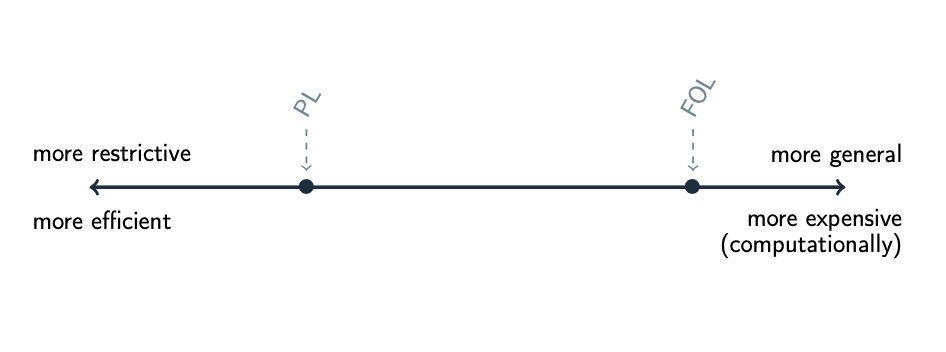
\includegraphics[height=5cm]{figures/tradeoff2.png}
    	Tradeoff propositional logic and first-order logic
    	\label{fig:tradeoff2}
    \end{figure}
    
    \newpage
    \item[--] \textbf{Extensions (make modelling more convenient)}
    \begin{itemize}
        \item[$\circ$] Sorts
        \begin{itemize}
            \item Intuitively: types of 'variables'
            \item E.g. numbers ($\forall x \in \mathbb{N}.\varphi)$, sets, lists
        \end{itemize}
        \item[$\circ$] Additional (abbreviations for) quantifiers
        \begin{itemize}
            \item E.g. 'there exists exactly one x such that ..": \\
            
            $\exists !x.\varphi(x) = \exists x.(\varphi(x) \wedge \forall y.(\varphi(y) \rightarrow (x = y)))$
        \end{itemize}
    \end{itemize}
    \vspace{0.2cm}
    \item[--] \textbf{Noteworthy}: reasoning over computer programs can be expressed using FOL
    \begin{itemize}
        \item[$\circ$] \textcolor{PineGreen}{Equivalence}: Given two computer programs $P_1, P_2$ do they compute the same outcome for each possible input?
        \item[$\circ$] \textcolor{PineGreen}{Termination}: Given a computer program $P$, for each possible input does it eventually terminate?
        \item[$\circ$] \textcolor{PineGreen}{Correctness}: Given a computer program $P$ and a specification of a function f, does $P$ compute the function f?
    \end{itemize}
    \item[--] For example, \textcolor{PineGreen}{Turing machines} (math. model of computation) can be encoded into \textcolor{red}{First-order logic}

\end{itemize}

\subsection{Second-order Logic (SOL)}
\begin{itemize}
    \item[--] \textbf{SOL} has \textbf{quantification} over relations: e.g., $\exists R . \forall x . \exists y . R(x,y)$
    \item[--] \textcolor{red}{Monadic Second-order Logic (MSOL)} is an often considered variant where second-order quantification is only over unary predicates
\end{itemize}

\subsection{Uncomputability}
\begin{itemize}
    \item[--] Main notion in the field of \textbf{Recursion theory}. 
    \item[--] A function $f: X \rightarrow Y$ is \textcolor{PineGreen}{computable} if there exists a computer program $P$ that computes this function f 
    \begin{itemize}
        \item[$\circ$] For each input $x \in X$, running $P$ on input $x$:
        \begin{enumerate}
            \item terminates, and
            \item gives as output $f(x)$
        \end{enumerate}
    \end{itemize}
    \subsubsection{Halting Problem (Alan Turing, 1936)} 
    Example of an uncomputable function:
    \begin{itemize}
        \item[$>$] \textbf{Input}: a computer program $P$ (Turing machine) and an input x
        \item[$>$] \textbf{Output}: does $P$, when run on x as input, eventually terminate (halt)?
    \end{itemize}
    \newpage
    \item[--] \textcolor{red}{Satisfiability} of First-order Logic:
    \begin{itemize}
        \item[$>$] \textbf{Input}: a first-order logic formula $\varphi$
        \item[$>$] \textbf{Output}: does there exist an interpretation $(l, \cdot^l)$ that satisfies $\varphi$?
        \\
        \item[$>$] \textbf{\textcolor{red}{Uncomputable!}}
        \item[$>$] e.g. there exists no algorithm that for each FOL formula $\varphi$ correctly tells us whether $\varphi$ is satisfiable (and that always gives an answer).
        \item[$>$] Similarly for the problems of \textcolor{PineGreen}{validity}, \textcolor{PineGreen}{equivalence} and \textcolor{PineGreen}{logical entailment}
    \end{itemize}
\end{itemize}

\textbf{FOL validities can be enumerated:}
\begin{itemize}
    \item[--] We can \textcolor{PineGreen}{enumerate} all valid first-order logic sentences
    \subsubsection{Gödel's Completeness Theorem (1929)}
    \begin{itemize}
        \item[$\circ$] All valid first-order logic formulas can be proven
        \begin{itemize}
            \item A formula $\varphi$ is \textcolor{PineGreen}{valid} if every interpretation $(l, \cdot^l)$ satisfies $\varphi$. \\
            In other words, $\varphi$ is \textcolor{PineGreen}{valid} iff $\neg \varphi$ is \textbf{not satisfiable}.
        \end{itemize}
        \item[$\circ$] In an appropriate proof system
    \end{itemize}
    \item[--] We can go over all possible proofs one-by-one. \\
    If there is a proof of $\varphi$, then we will find it after some finite amount of time.
\end{itemize}

\textbf{Restrictions of FOL:} \\
\begin{itemize}
    \item[--] FOL is \textcolor{red}{too powerful} to effectively reason with algorithmically, in general.
    \item[--] To enable algorithms that always give the correct answer, restrictions are considered, e.g.:
    \begin{itemize}
        \item[$\circ$] Only allow formulas of a particular form (e.g., the \textcolor{Magenta}{guarded fragment} of FOL)
        \item[$\circ$] Languages that contain only some operators from FOL (and that sometimes look a bit different; e.g., \textcolor{Maroon}{description logics})
    \end{itemize}
\end{itemize}

\subsection{Computational complexity}
Computational Complexity is a part of theoretical computer science and studies how much resources (e.g., time, space) you need to solve computational problems.
\begin{itemize}
    \item[--] "Is there an algorithm for this problem that is guaranteed to be efficient?"
    \item[--] Measures the amount of time/space in terms of the length of the input.
\end{itemize}

\textbf{Main method}: categorizing computational problems into \textcolor{PineGreen}{complexity classes}

\begin{itemize}
    \item[--] \textbf{\textcolor{PineGreen}{Polynomial-time solvability}} is the typical notion of "efficiently solvable"
    \begin{itemize}
        \item[$\circ$] An algorithm runs in polynomial time if there is a polynomial function $p(n)$ such that on \textbf{any} input (of length n), the algorithm terminates within at most $p(n)$ time steps. E.g., $p(n) = 2n$, or $p(n) = 10n^2 + 100n$ 
    \end{itemize}
    \item[--] The complexity class \textcolor{red}{P} contains problems that are solvable in polynomial time.
    \item[--] The complexity class \textcolor{NavyBlue}{NP} contains problems where:
    \begin{itemize}
        \item[$\circ$] the goal is to find a solution in a search space that is of exponential size (in the input size $n$);
        \item[$\circ$] for each candidate solution, you can efficiently (in polynomial time) check whether or not it is a correct solution.
    \end{itemize}
    \item[--] An example of an NP problem is \textcolor{PineGreen}{satisfiability for propositional logic (SAT)}.
    \item[--] Best alg. for hard problems in NP take \textbf{\textcolor{red}{exponential time}}, in the \textbf{worst case}.
    \item[--] \textbf{More complexity classes:}
    \begin{itemize}
        \item[$\square$] \textbf{PSPACE}: problems that can be solved with polynomial memory usage (possibly exponential time).
        \item[$\square$] \textbf{EXP}: problems that can be solved within exponential time (possibly exponential memory usage).
        \item[$\square$] \textbf{EXPSPACE}: problems that can be solved with exponential memory usage (possibly doubly-exponential time).
    \end{itemize}
\end{itemize}

\subsection{Monotonicity}
Propositional logic and first-order logic are \textbf{\textcolor{red}{monotonic}} in the following sense:
\begin{itemize}
    \item[--] Take some formula $\varphi_1$
    \item[--] Suppose that I can derive some conclusion from it: $\varphi \models \psi$
    \item[--] Now if I add further information to my formula: $\varphi_1 \wedge \varphi_2$
    \item[--] Then I can always still derive the original conclusion: $\varphi_1 \wedge \varphi_2 \models \psi$
\end{itemize}

For some types of applications, \textbf{non-monotonic reasoning} is \textbf{desirable}:
\begin{itemize}
    \item \textbf{\textcolor{PineGreen}{Non-monotonicity}}: "new information can cause me to retract previous conclusions".
    \item It can be that $\varphi_1 \models \psi$ but $\varphi_1 \wedge \varphi_2 \not \models \psi$.
\end{itemize}

\textbf{For example}:
\begin{itemize}
    \item "Given evidence E, the most likely explanation of something is X"
    \item "With new evidence, so $E \cup E^\prime $, the most likely explanation now is $X^\prime \neq X$ ".
\end{itemize}

Non-monotonicity is another feature on the wish list for knowl. repr. languages.